\usetikzlibrary{arrows.meta,calc}
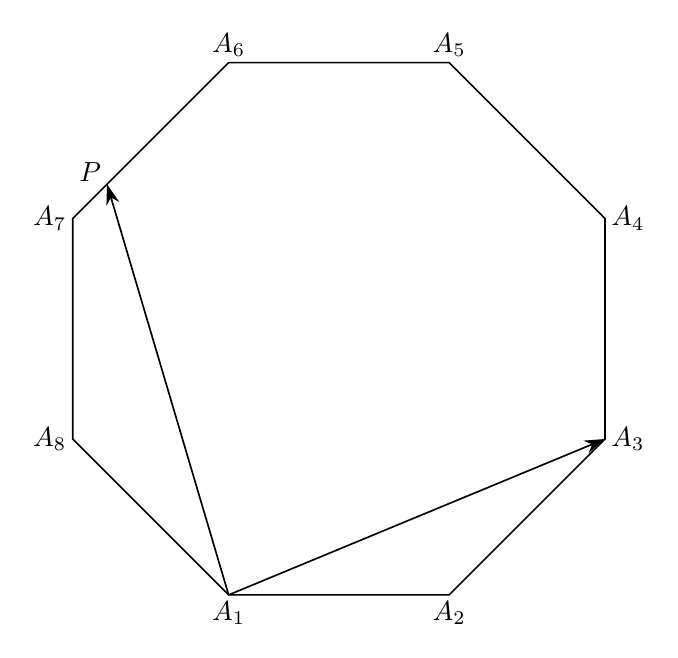
\begin{tikzpicture}[x=1cm,y=1cm,line width=.6pt,>=Stealth,
  geometry edge/.style={solid,line width=.6pt},
  geometry label/.style={font=\normalsize,inner sep=2pt},
  vector/.style={-{Stealth[length=2.6mm,width=1.7mm]},line width=.6pt}]
\coordinate (A1) at (0,0);
\coordinate (A2) at (2.8,0);
\coordinate (A3) at (4.779899,1.979899);
\coordinate (A4) at (4.779899,4.779899);
\coordinate (A5) at (2.8,6.759798);
\coordinate (A6) at (0,6.759798);
\coordinate (A7) at (-1.979899,4.779899);
\coordinate (A8) at (-1.979899,1.979899);
\coordinate (P) at (-1.544321,5.215477);
\draw[geometry edge] (A1)--(A2)--(A3)--(A4)--(A5)--(A6)--(A7)--(A8)--cycle;
\draw[vector] (A1)--(A3);
\draw[vector] (A1)--(P);
\node[geometry label,below] at (A1) {$A_1$};
\node[geometry label,below] at (A2) {$A_2$};
\node[geometry label,right] at (A3) {$A_3$};
\node[geometry label,right] at (A4) {$A_4$};
\node[geometry label,above] at (A5) {$A_5$};
\node[geometry label,above] at (A6) {$A_6$};
\node[geometry label,left] at (A7) {$A_7$};
\node[geometry label,left] at (A8) {$A_8$};
\node[geometry label] at (-1.76,5.37) {$P$};
\end{tikzpicture}
